\documentclass{article}
\usepackage[utf8]{inputenc}
\usepackage[T2A]{fontenc}
\usepackage[russian]{babel}
\usepackage{amsfonts}
\usepackage{amsmath}
\usepackage{amssymb}
\usepackage{arcs}
\usepackage{fancyhdr}
\usepackage{float}
\usepackage[left=3cm,right=3cm,top=3cm,bottom=3cm]{geometry}
\usepackage{graphicx}
\DeclareGraphicsExtensions{.png}
\usepackage{hyperref}
\usepackage{multicol}
\usepackage{stackrel}
\usepackage{xcolor}
\usepackage{minted}

\begin{document}
\title{Отчет по лабораторной работе 6}
\date{}
\maketitle

\subsubsection*{Параметры виртуальной машины, на которой проводился эксперимент:}
\begin{itemize}
    \item Общий объем оперативной памяти: 4005120 kB;
    \item Объем раздела подкачки: 4004860 kB;
    \item Размер страницы виртуальной памяти: 4 kB;
    \item Процессор: по умолчанию в UTM с количеством ядер, указанном в эксперименте.
\end{itemize}

\subsubsection*{Параметры хостового компьютера, на котором проводился эксперимент:}
\begin{itemize}
    \item Общий объем оперативной памяти: 16777216 kB;
    \item Процессор: Apple M1, 8‑ядерный процессор с 4 ядрами производительности и 4 ядрами эффективности.
\end{itemize}

\bigskip

\subsection*{Эксперимент №1}
За сложный алгоритм было взято вычисление геометрического ряда Маклорена: 

\medskip 

\noindent $\dfrac{1}{1 - x} = 1 + x + x^{2} + x^{3} + \dots + x^{n}, \; |x| < 1$. 

\medskip

\noindent Время выполнения для любого входного параметра составляет 3 секунды при использовании 1 ядра. Реализацию можно посмотреть в файле \textbf{function.sh}.

\subsubsection*{Последовательный запуск программы с использованием 1 ядра}
Реализация скрипта, выполняющего последовательно $N$ вычислений, находится в файле \textbf{1\_1b.sh}. \\
Реализация скрипта, выполняющего 10 запусков для $N$ в диапазоне от 1 до 20, находится в файле \textbf{1\_1c.sh}. \\
Данные записывались в файл \textbf{log\_1\_1}, после чего были посчитаны средние значения, которые отображены на Рис.1.

\subsubsection*{Параллельный запуск программы с использованием 1 ядра}
Реализация скрипта, выполняющего параллельно $N$ вычислений, находится в файле \textbf{1\_2a.sh}. \\
Реализация скрипта, выполняющего 10 запусков для $N$ в диапазоне от 1 до 20, находится в файле \textbf{1\_2b.sh}. \\
Данные записывались в файл \textbf{log\_1\_2}, после чего были посчитаны средние значения, которые отображены на Рис.2.

\subsubsection*{Последовательный запуск программы с использованием 2 ядер}
Необходимые скрипты уже реализованы. \\
Данные записывались в файл \textbf{log\_1\_3}, после чего были посчитаны средние значения, которые отображены на Рис.3.

\subsubsection*{Параллельный запуск программы с использованием 2 ядер}
Необходимые скрипты уже реализованы. \\
Данные записывались в файл \textbf{log\_1\_4}, после чего были посчитаны средние значения, которые отображены на Рис.4.

\bigskip

\subsection*{Эксперимент №2}
Для описанного алгоритма было реализовано 2 скрипта: \textbf{create\_files.sh}, который создает необходимые файлы, и \textbf{write.sh}, который для каждого числа в файле записывает в конец удвоенное значение.

\subsubsection*{Последовательный запуск программы с использованием 1 ядра}
Реализация скрипта, выполняющего последовательно $N$ вычислений, находится в файле \textbf{2\_1b.sh}. \\
Реализация скрипта, выполняющего 10 запусков для $N$ в диапазоне от 1 до 20, находится в файле \textbf{2\_1c.sh}. \\
Данные записывались в файл \textbf{log\_2\_1}, после чего были посчитаны средние значения, которые отображены на Рис.5.

\subsubsection*{Параллельный запуск программы с использованием 1 ядра}
Реализация скрипта, выполняющего параллельно $N$ вычислений, находится в файле \textbf{2\_2a.sh}. \\
Реализация скрипта, выполняющего 10 запусков для $N$ в диапазоне от 1 до 20, находится в файле \textbf{2\_2b.sh}. \\
Данные записывались в файл \textbf{log\_2\_2}, после чего были посчитаны средние значения, которые отображены на Рис.6.

\subsubsection*{Последовательный запуск программы с использованием 2 ядер}
Необходимые скрипты уже реализованы. \\
Данные записывались в файл \textbf{log\_2\_3}, после чего были посчитаны средние значения, которые отображены на Рис.7.

\subsubsection*{Параллельный запуск программы с использованием 2 ядер}
Необходимые скрипты уже реализованы. \\
Данные записывались в файл \textbf{log\_2\_4}, после чего были посчитаны средние значения, которые отображены на Рис.8.

\bigskip

\subsection*{Вывод}

\subsubsection*{Эксперимент №1}
\begin{itemize}
    \item Все 4 графика показали линейный рост;
    \item При использовании одного ядра и последовательном запуске время выполнения (с ростом значения $N$) увеличивалось, примерно, на время выполнения одного запуска (2-3 секунды);
    \item При использовании одного ядра и параллельном запуске время выполнения (с ростом значения $N$) увеличивалось аналогично. Никакого выигрыша параллелизм не дал;
    \item При использовании двух ядер и последовательном запуске время выполнения (с ростом значения $N$) увеличивалось аналогично. Увеличение числа ядер не дало выигрыша при последовательном выполнение программы;
    \item При использовании двух ядер и параллельном запуске время выполнения (с ростом значения $N$) увеличивалось вдвое меньше, чем в предыдущих разах. Параллельные запуски с большим количеством ядер дают выигрыш во времени.
\end{itemize}

\subsubsection*{Эксперимент №2}
\begin{itemize}
    \item Все 4 графика показали линейный рост;
    \item При использовании одного ядра и последовательном запуске время выполнения (с ростом значения $N$) увеличивалось, примерно, на время выполнения одного запуска (2-3 секунды);
    \item При использовании одного ядра и параллельном запуске время выполнения (с ростом значения $N$) оказалось даже больше, чем при последовательном запуске. Параллельный запуск оказался хуже при 1 ядре;
    \item При использовании двух ядер и последовательном запуске время выполнения (с ростом значения $N$) уменьшилось. Увеличение ядер снизило время выполнения программы;
    \item При использовании двух ядер и параллельном запуске время выполнения (с ростом значения $N$) уменьшилось еще больше. Тем самым, получили значительный выигрыш во времени выполнения программы при использовании большего количества ядер и параллелизма.
\end{itemize}

\newpage

\begin{figure}
    \centering
    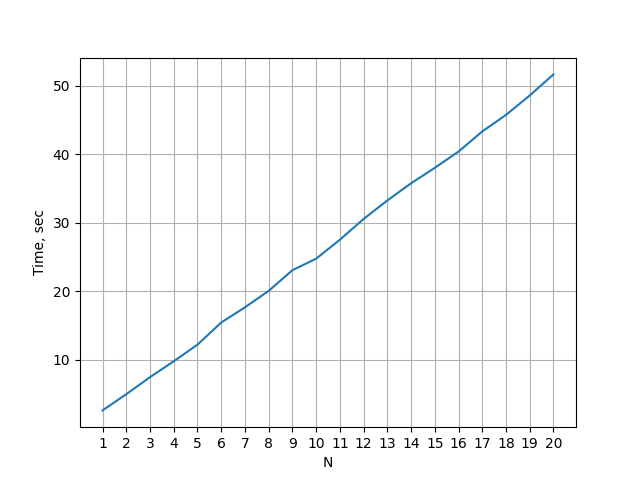
\includegraphics[scale=0.7]{Graphic-1.png}
    \caption{Эксперимент №1, последовательный запуск, 1 ядро}
    \label{fig:enter-label}
\end{figure}

\begin{figure}
    \centering
    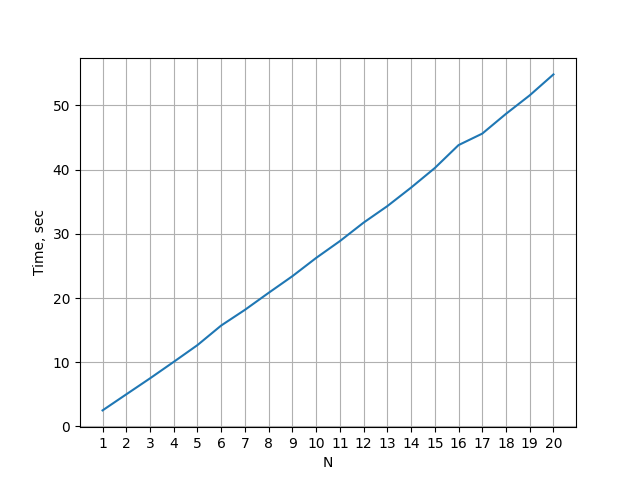
\includegraphics[scale=0.7]{Graphic-2.png}
    \caption{Эксперимент №1, параллельный запуск, 1 ядро}
    \label{fig:enter-label}
\end{figure}

\begin{figure}
    \centering
    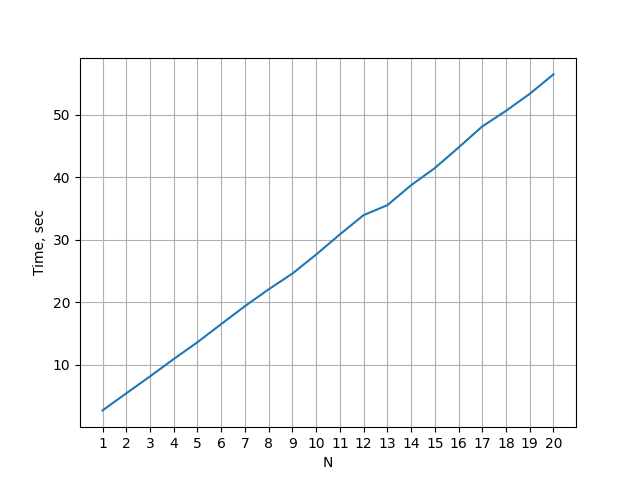
\includegraphics[scale=0.7]{Graphic-3.png}
    \caption{Эксперимент №1, последовательный запуск, 2 ядра}
    \label{fig:enter-label}
\end{figure}

\begin{figure}
    \centering
    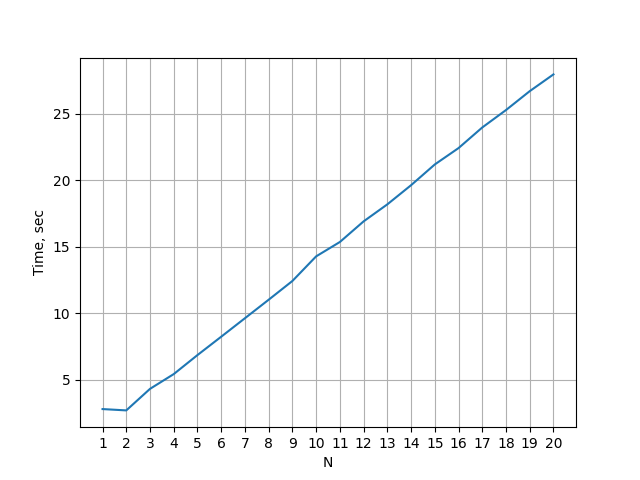
\includegraphics[scale=0.7]{Graphic-4.png}
    \caption{Эксперимент №1, параллельный запуск, 2 ядра}
    \label{fig:enter-label}
\end{figure}

\begin{figure}
    \centering
    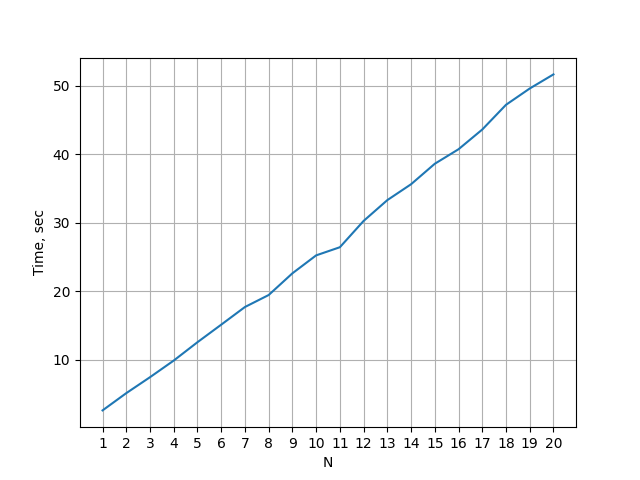
\includegraphics[scale=0.7]{Graphic-5.png}
    \caption{Эксперимент №2, последовательный запуск, 1 ядро}
    \label{fig:enter-label}
\end{figure}

\begin{figure}
    \centering
    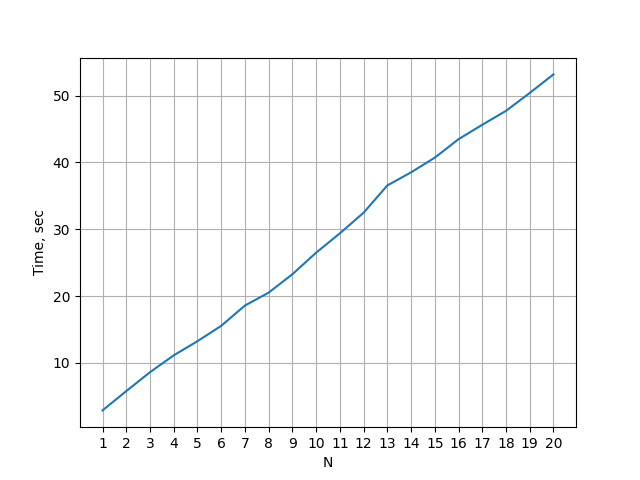
\includegraphics[scale=0.7]{Graphic-6.png}
    \caption{Эксперимент №2, параллельный запуск, 1 ядро}
    \label{fig:enter-label}
\end{figure}

\begin{figure}
    \centering
    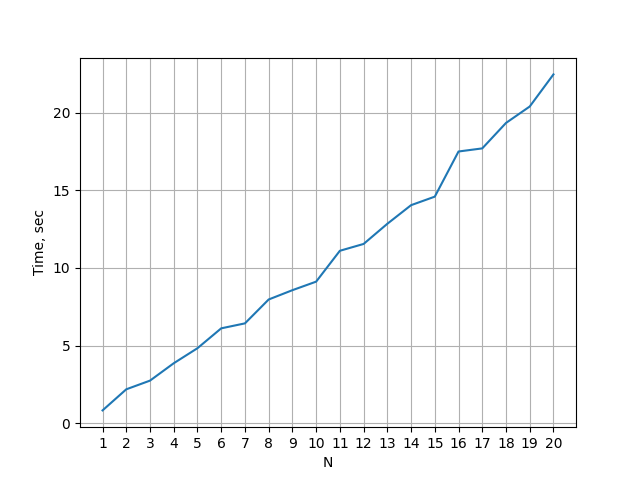
\includegraphics[scale=0.7]{Graphic-7.png}
    \caption{Эксперимент №2, последовательный запуск, 2 ядра}
    \label{fig:enter-label}
\end{figure}

\begin{figure}
    \centering
    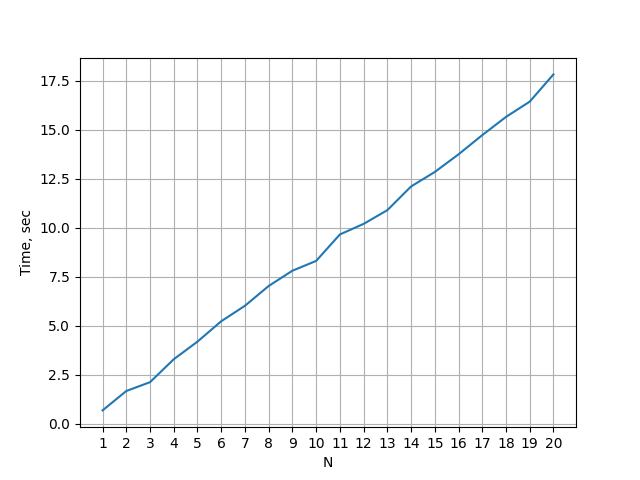
\includegraphics[scale=0.7]{Graphic-8.png}
    \caption{Эксперимент №2, параллельный запуск, 2 ядра}
    \label{fig:enter-label}
\end{figure}

\end{document}
